\documentclass{acm_proc_article-sp}
\usepackage{algorithmic}
\usepackage{algorithm}

\begin{document}

\title{Reward-Based Social Learning}

\numberofauthors{3}
\author{
\alignauthor
Wesley Tansey\\
       \affaddr{Dept. of Computer Science, The University of Texas at Austin}\\
       \affaddr{1 University Station C0500, Austin, TX, USA}\\
       \email{tansey@cs.utexas.edu}
\alignauthor
Eli Feasley\\
       \affaddr{Dept. of Computer Science, The University of Texas at Austin}\\
       \affaddr{1 University Station C0500, Austin, TX, USA}\\
       \email{elie@cs.utexas.edu}
\alignauthor
Risto Miikkulainen\\
       \affaddr{Dept. of Computer Science, The University of Texas at Austin}\\
       \affaddr{1 University Station C0500, Austin, TX, USA}\\
       \email{risto@cs.utexas.edu}
}
\date{25 January 2012}

\maketitle
\begin{abstract}
Social learning is an extension to evolutionary algorithms that enables agents to learn from observations of others in the population. Traditionally, social learning algorithms have employed a student-teacher model where the behavior of one or more high-fitness agents is used to train a subset of the remaining agents in the population. We present a reward-based model of social learning in which agents are not labeled as teachers or students, instead allowing any individual receiving a sufficiently high reward to teach other agents to mimic its recent behavior. We validate our approach through a series of experiments in a robot foraging domain, including comparisons of reward-based social learning with pure neuroevolution and a variant of student-teacher social learning. We show that our algorithm converges to near-optimal strategies faster than either benchmark approach, outperforming both in a complex foraging task by more than an order of magnitude. Our results suggest reward-based social learning holds substantial potential to revolutionize the field of social learning.
\end{abstract}

\terms{Social Learning, Evolutionary Algorithms, Artificial Life}

\section{Introduction}

One explanation for the evolution of large brains in primates is the social intelligence hypothesis, which states that the selection pressure driving the increase in brain size was the need to handle complex social behaviors. The cultural intelligence hypothesis extends this concept solely to humans, stating that our brains evolved to handle the specific challenge of culture creation and social learning. These hypotheses are currently the most widely accepted explanations for the evolution of the human brain among evolutionary biologists and cognitive scientists \cite{holekamp2007questioning}, and has been supported by strong empirical evidence in recent years \cite{herrmann2007humans}.

Cultural and social learning algorithms \cite{reynolds1994introduction} model this biological mechanism in multi-agent systems by designating teacher agents that propagate knowledge and train other agents in the population. These techniques effectively enhance Evolutionary Algorithms (EAs) with a hierarchical structure (i.e., students and teachers) that facilitates the automatic discovery of suitable actions to use as training examples and target individuals to train. Thus, while cultural algorithms capture the ability of humans to learn from formal instruction, they do not fully model all forms of learning from observation in primates.

We present a reward-based approach to social learning, inspired by mirror neurons \cite{gallese-98}, in which agents learn by observing the actions of other individuals. Primate brains contain mirror neurons that activate when other primates are observed, in effect mirroring the observed primate's action internally. Analogously, agents in our algorithm observe the population and, when a positive reward is received, mimic that action in order to learn a policy similar to that of the observed agent. This algorithm separates itself from other social learning algorithms in that the quality of a training example is measured by the reward received rather than the hierarchical role of the agent generating the example.

We validate our algorithm in a well-known foraging domain in which agents must discriminate between poisonous and nutritious food. \textit{Summarize results section here}

This paper makes the following novel contributions:
 
\begin{itemize}
\item A reward-based approach to social learning, in which individuals are not classified into roles.
\item An exploration of the role of filtering by rewarded examples and by similarity between agents.
\item An analysis of the differences in performance between reward-based social learning and traditional student-teacher social learning
\end{itemize}
 
The remainder of the paper is structured as follows.
In Section \ref{sec:rbsl} we detail the workings of our reward-based social learning algorithm.
Prior work is discussed in Section \ref{sec:background}.
In Section \ref{sec:setup} we describe our experimental setup and the foraging domain.
Section \ref{sec:results} presents the results of our experiments.
Planned extensions to our work are described in Section \ref{sec:future}. Finally, in Section \ref{sec:conclusions} we present our conclusions.

\section{Background}
\label{sec:background}
In this section, we provide background information and motivation for social learning, and introduce our evolutionary framework, Neuroevolution of Augmented Topologies (NEAT).

\subsection*{Social Learning}

In this section, we elaborate on our approach and its justification and applications. First, we discuss some of the advantages of reward-based social learning and the domains in which it provides promising functionality. Next, we describe the algorithm at the core of our model. Finally, we go into some detail about the particulars of our implementation.

Social learning is valuable in expensive domains; when computing time is limited or individuals have limited experiential training data, leveraging the experiences of multiple individuals is a valuable way to use the information that is available. As video games and real-life applications of intelligent agents become more pervasive, these expensive-to-simulate, easy-to-record domains are becoming more and more common. Every agent can benefit from the experiences of every other without the expense of rerunning the training environment.

Another important area for social learning is dynamic domains. In multiagent systems, changing conditions can negatively impact all agents if they cannot learn from one another's experience - but if they can, one agent's experience of a novel stimulus can alert other agents so they can adjust their behavior. If a social learning system is on-line, sharing updates and information about reward at every timestep, adaptation can occur rapidly.


\subsection*{Evolutionary Framework}
In this section, we discuss the framework on which we base our social learning and our modifications and extensions to this framework.

NeuroEvolution of Augmented Topologies (NEAT)\cite{stanley2002evolving} is an evolutionary algorithm that generates recurrent neural networks. Through a process of adding and removing nodes and changing weights, NEAT evolves genomes that unfold into networks. In every generation, those networks with the highest fitness reproduce, and those that have low fitness are less likely to do so. NEAT maintains genetic diversity through speciation and encourages innovation through explicit fitness sharing.

In our domain, NEAT is used to generate a population of individual neural networks that control agents in the world. The input to each network is the agent's sensors, and the outputs control the agent's velocity and orientation. The fitness of each network is determined by the success of the agent it controls - over the course of a generation, networks controlling agents who eat a good deal of rewarding food and very little poison will have high fitnesses and those which control agents with less wise dietary habits will have low fitness.

In standard NEAT, the networks that are created do not change within one generation, but in reward-based social learning, we do backpropagation\cite{rumelhart1986learning} on the networks that NEAT creates. (Because these networks are recurrent, we use backpropagation through time to do our social learning \cite{werbos1990backpropagation}.) The final fitness of each phenome, then, reflects the performance of the individual that used that phenome and elaborated on it over the course of a generation. In Darwinian evolution, the changes that were made to the phenome over the course of a generation are not saved; in Lamarkian, the genome itself is modified.

\subsection*{Previous Work}

Enhancing EAs with social and cultural learning is a flourishing area of research with a long and successful track record. We next highlight relevant prior work and explain how our approach differs from previous efforts.

Cultural algorithms \cite{reynolds1994introduction} have been used frequently in Particle Swarm Optimization (PSO) \cite{kennedy1995particle}. These algorithms maintain a ``belief space'' representing different categories of knowledge that the population has learned. New individuals are trained using this belief space in a student-teacher paradigm. In contrast, our agents maintain no separate repository of formal knowledge, but rather they learn from observations of others during their lifetime.

Interestingly, our approach could be seen as a Memetic Algorithm (MA) \cite{moscato1989evolution}. As originally defined by Dawkins \cite{dawkins2006selfish}, a meme is a ``unit of imitation in cultural transmission'' including ``tunes, ideas, catch-phrases, clothes fashions, ways of making pots or of building arches''. Our approach particularly relates to the latter--- ways of making pots or building arches are similar to learning strategies for gathering food in that all are instances of transmitting specific strategies for performing skilled tasks. Thus, each reward-based learning example could be considered as a meme being shared within the agent's population or cultural group. Nevertheless, traditional MAs \cite{onwubolu2004new}, including similar Lamarkian evolution methods for evolving recurrent neural networks \cite{ku2000study}, focus on using local improvement heuristics and typically rely on off-line transmission of memes via mating and genetic recombination. However, agents in our approach transmit memes on-line, as they are generated and observed during the evaluation process. Thus, while we could classify our approach as an MA, we believe the distinct transmission and learning techniques employed by our algorithm better characterize it as a social learning method.

The ability of social learning to improve agents in a foraging domain has been explored by several researchers in recent years. Denaro et. al. \cite{denaro1996cultural} used a student-teacher model of cultural evolution without genetic inheritance and demonstrated that the population will continue to improve if Gaussian noise is added to the training examples. The NEW TIES system \cite{haasdijk2008social, vogt2010modeling} simulates a steady state evolution of decision tree agents where at each step the teacher agents probabilistically transmit their decisions and students probabilistically incorporate this knowledge. Acerbi et. al. \cite{acerbi2007social} use social learning to train embodied agents to mimic the behaviors of more experienced agents. Finally, de Oca et. al. \cite{de2011incremental} propose a methodology for incremental social learning in PSO to update Q-learning \cite{watkins1992q} value functions by randomly selecting two individuals from the population and combining their values for a given update. While all of these works are closely related and motivated by similar biological processes as our approach, they fundamentally all rely on the concept of students and teachers, and perform either no filtering or a reward-agnostic filtering of state-action pairs to be used in updating the population.


\section{Reward-Based Social Learning}
\label{sec:rbsl}

Our approach, detailed in Figure \ref{fig:flowchart} is an on-line learning algorithm that operates continuously as an agent moves in the world. At every timestep, each agent perceives the state of the world around it, and activates an internal neural network according to that state. The output of this network represents the agent's motor commands. Both the input and the output of the network are saved and stored in memory. Upon moving, an agent encountering a positive reward will retrieve its recent inputs and associated outputs from memory and train other individuals on these input-output pairs using backpropagation.

\begin{algorithm}
\caption{Our Reward-Based Learning Algorithm}
\label{reward-algo}
\begin{algorithmic}
\STATE \textbf{Input:} $generations, maxTimesteps$
\STATE $population \leftarrow$InitializePopulation()
\STATE $g \leftarrow 0$
\STATE $t \leftarrow 0$
\LOOP
\WHILE{$g < generations$}
  \STATE $cliques \leftarrow$ FormCliques($population$)
  \WHILE{$t < maxTimesteps$}
    \FOR{each $clique$ in $cliques$}
      \FORALL{$agents$ in $clique$}
        \STATE $state \leftarrow $ReceiveAgentInputs()
        \STATE $action \leftarrow $Activate($agent.network$)
        \STATE $agent.memory \leftarrow (state, action)$
        \STATE $agent.reward \leftarrow $TakeAction(action)
      \ENDFOR
    \FORALL{$agents$ in $clique$}
      \IF{$agent.reward > 0$}
        \FORALL{$observer$ in $clique$}
          \STATE Train($observer, agent.memory$)
        \ENDFOR
      \ENDIF
    \ENDFOR
    \ENDFOR
    \STATE $t \leftarrow t + 1$
  \ENDWHILE
  \STATE $population \leftarrow$SelectAndReproduce($population$)
  \STATE $g \leftarrow g + 1$
\ENDWHILE
\ENDLOOP
\end{algorithmic}
\end{algorithm}

\begin{figure}
  \centering
    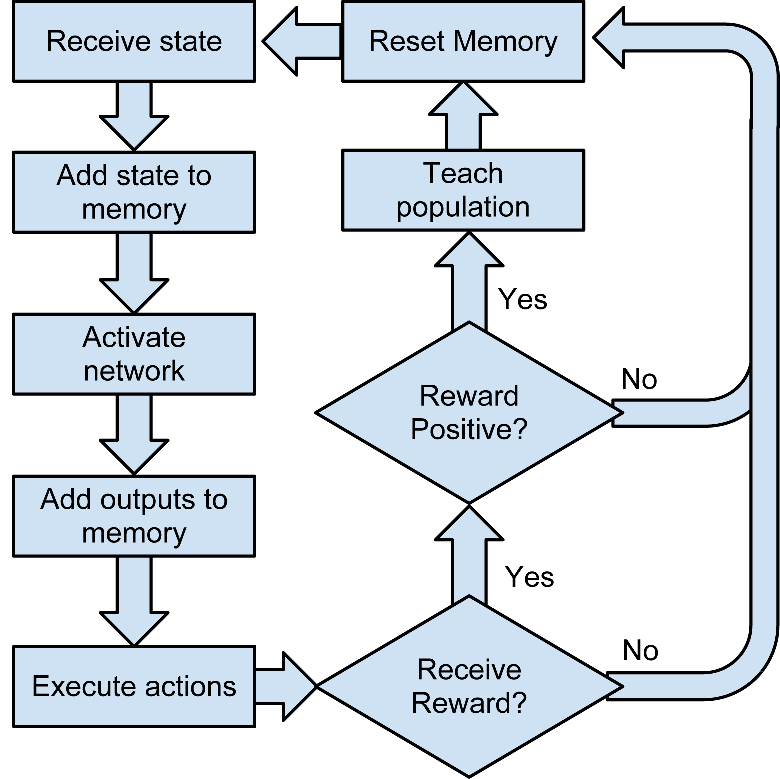
\includegraphics[scale=.6]{flowchart.pdf}
  \caption{Individuals remember their most recent inputs and the associated actions taken, and when rewarded will train other individuals on their recent actions.}
  \label{fig:flowchart}
\end{figure}


As a result of using only positive rewards to identify those actions on which we want to train agents, social learning can begin immediately in the first generation of the evolutionary algorithm. In contrast, previous approaches \cite{denaro1996cultural} instead chose strong individuals as teachers to train weaker individuals in appropriate behavior, thereby requiring at least one generation in which to identify strong individuals. Additionally, by allowing any individual to train any other, we leverage a diversity of different behaviors in problem solving.

\section{Experimental Setup}
\label{sec:setup}
In this section we describe our evaluation domain, including the inputs and outputs that our agents receive, and the common parameters across all our experiments.


\begin{figure}[t]
  \centering
    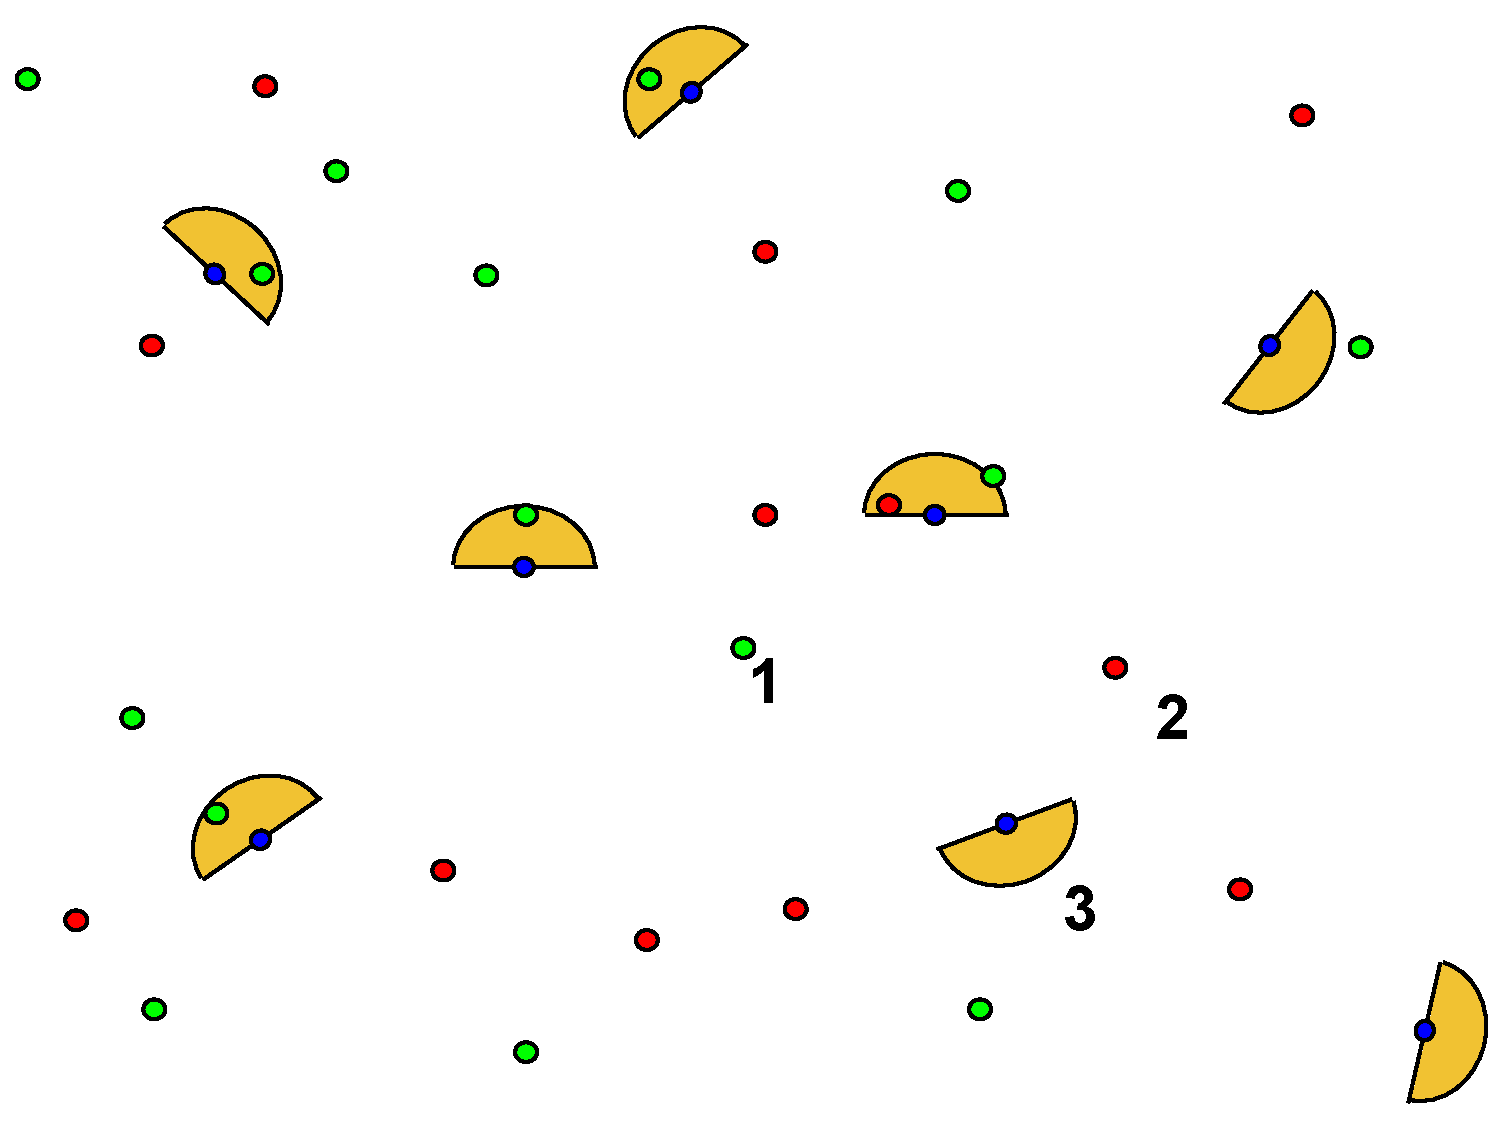
\includegraphics[scale=.31]{world.pdf}
  \caption{Our domain: a foraging world in which agents gain fitness by consuming plants which they approach.  \textbf{1} is a piece of nutritious food which increases fitness, \textbf{2} is poison which decreases fitness, and \textbf{3} is one of our agents.}
  \label{fig:foraging-world}
\end{figure}

\subsection*{The Foraging Domain}
Our domain is a foraging world in which agents move freely on a continuous toroidal surface. We populate our world with various plants, some of which are nutritious and bear positive reward, while others are poisonous and bear negative reward. These plants are randomly distributed over the surface of the world. The foraging domain is non-competitive and non-cooperative; each agent acts independently of all other agents, with the exception of the teaching signals which pass between them. At the start of each generation, all individuals begin at the center of the world, oriented in the same direction, and confronted with the same plant layout and configuration. Every agent then has a fixed number time steps to move about the surface of the world eating plants--- which happens automatically when an agent draws sufficiently close to one--- before the evaluation is over. Figure \ref{fig:foraging-world} shows an example of a foraging world with two types of plants and eight agents.
    
\begin{figure}[t]
  \centering
    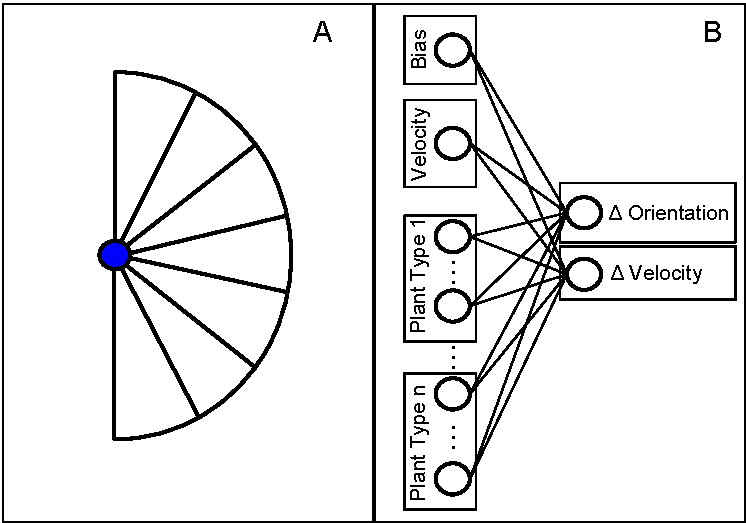
\includegraphics[scale=.665]{foraging_agent_architecture.pdf}
  \caption{The architecture of our foraging agents. A) Each agent has a 180$^{\circ}$ field of vision, discretized into eight sensors for each plant type. B) Each agent is controlled by a neural network taking the agent's current velocity and sensor activations as inputs and outputting the desired change in orientation and velocity.}
  \label{fig:agent-architecture}
\end{figure}

\subsection*{Sensors and Outputs}

Agents ``see'' plants within a 180$^\circ$ horizon via a collection discretized sensors. Each agent has eight sensors for each type of plant, each of which detects plants in a different 12.5 degree$^\circ$ sector of the 180$^\circ$ ahead of the agent. Agents cannot see other individuals, or plants they have already eaten--- all they can see is edible food. The strength of the signal generated by each plant is proportional to its proximity to the agent. Agents also have a sensor by which they can detect their current velocity. Each agent is controlled by an artificial neural network that maps from the agent's sensor readings to the desired change in orientation and velocity. Figure \ref{fig:agent-architecture} shows the architecture of a foraging agent.

\subsection*{Common Parameters}

In our experiments, we used two separate configurations for the robot foraging world. In the first three experiments, we used a ``simple'' world where the toroidal surface is 2000 by 2000 units, with a single plant type of value 100 and 50 randomly distributed instances of the plants. In this world, the agents have a straight-forward task of learning to efficiently navigate and gather as many plants as possible.

For our fourth set of experiments, we evaluated using both the simple world and a second, more complex world. Our ``complex'' world has a surface of 500 by 500 units, with five different plant types of value: $\{-100, -50, 0, 50, 100\}$. For each plant type, we create 20 randomly distributed plant instances. This world presents the agents with a more difficult task as they must both efficiently gather nutrious food while simultaneously avoiding the poisonous food.

In all our experiments, we create 100 different agents in each generation. All networks are initialized with fully-connected weights with no hidden neurons. Agents automatically eat any plant with which they are within five units. Each evaluation lasts 1000 timesteps and our results for each experiment are the average of 30 independent runs.

We next describe our experiments and their outcomes in detail.

%In both worlds, there are 100 agents and when they are divided into cultural cliques, there are ten cliques of ten agents. Each agent had 8 different sensors for each type of plant, and automatically ate any plant it came within 5 units of. 

\section{Results}
\label{sec:results}
In this section we present our experimental results. We conducted four main experiments, 1) determining the baseline performance of reward-based social learning and neuroevolution, each in isolation, 2) measuring the performance of reward-based learning in Darwinian and Lamarkian evolutionary paradigms, 3) evaluating whether cultural learning improves performance compared to having a mono-culture population, and 4) comparing reward-based learning to a student-teacher learning algorithm in both simple and complex foraging tasks. The first three experiments examine the efficacy of the various components of our algorithm while the fourth experiment serves as a validation for our final algorithm against a variant of a related approach in the literature. The results of our experiments show that our algorithm is able to evolve high-quality strategies with substantially less agent evaluations than previous algorithms.

%determining the feasibility of reward-based social learning in isolation without any evolution and establishing a baseline result for pure neuroevolution with no on-line learning

\begin{figure}
  \centering
    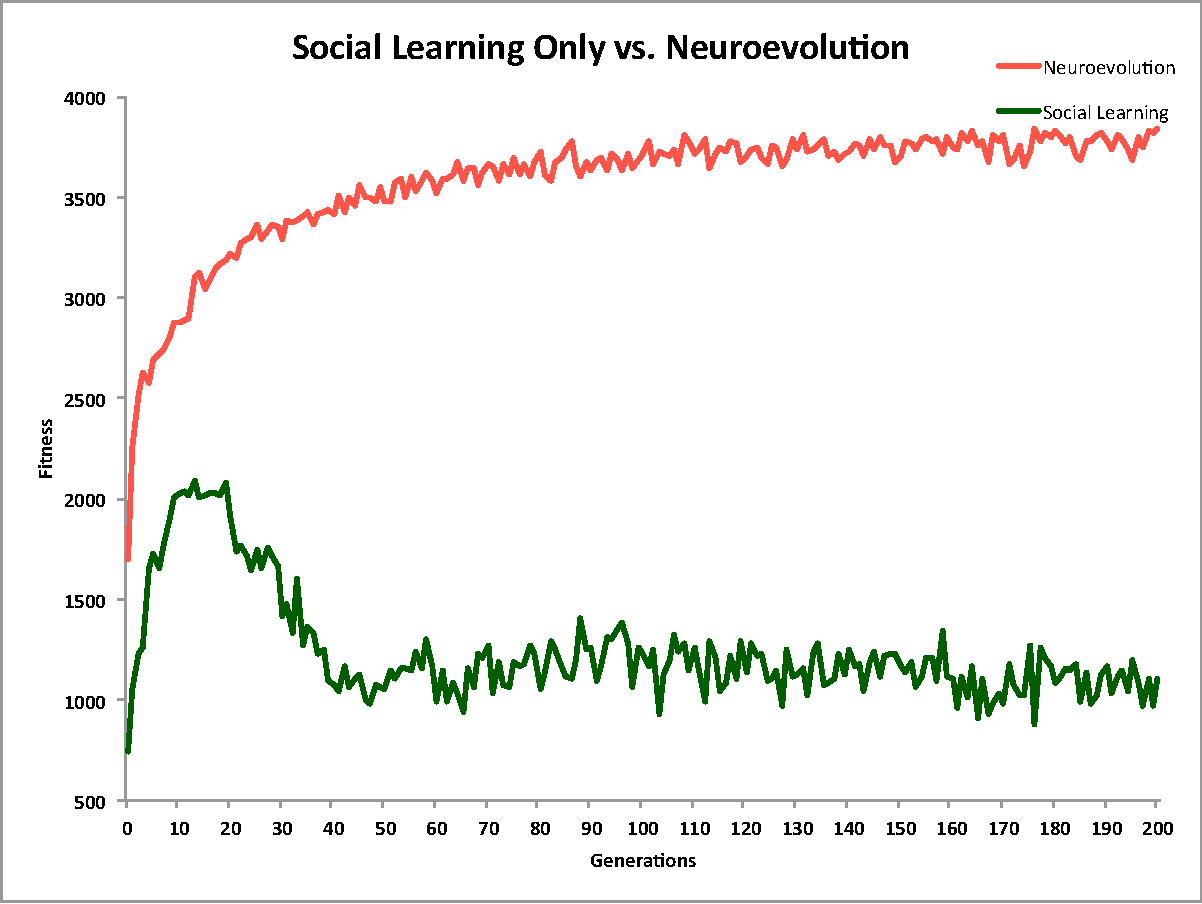
\includegraphics[scale=.35]{social_learning_vs_neuroevolution.pdf}
  \caption{Pure reward-based learning collapses after several generations, while neuroevolution alone converges to a stable but suboptimal solution.}
  \label{fig:social-neuro}
\end{figure}

\subsection*{Reward-Based learning vs. Neuroevolution}

We first wish to establish a baseline for understanding the ability of our two component methods, social learning and neuroevolution, to evolve high-quality strategies in isolation. To evaluate social learning in isolation, we created a population of 100 randomly initialized neural networks and evaluated them without selection or reproduction for 200K time steps. After every 1000 time steps, the population champion was recorded and this was treated as a ``generation'' in order to compare it to baseline neuroevolution.

Figure \ref{fig:social-neuro} shows the results of the experiment. While reward-based social learning alone is initially able to improve, after several epochs a regression to the mean effect is observed in which the entire population converges to a mediocre average score. A similar effect has been observed in previous social learning experiments \cite{denaro1996cultural}, suggesting that some form of mutation is needed to prevent population collapse. In contrast, neuroevolution converges to strong solutions with fitnesses of around 3500 after approximately 50 generations.

Having validated that social learning alone is not sufficient, we next compare the performance of social learning when used as an enhancement to evolution.


\subsection*{Darwinian vs. Lamarkian evolution}

Genetic inheritance paradigms in evolution fall into one of two main categories: Darwinian and Lamarkian. In Darwinian evolution, individual genomes are fixed and any knowledge or abilities gained during their lifetimes are not passed on to their offspring at birth. By contrast, in Lamarkian evolution an individual's genome changes as it learns throughout its life, and these changes are passed on to each of its offspring. In the context of our experiments, this corresponds to whether the changes in each individual's neural network weights, as a result of social learning, are propagated to their genome at the end of the generation.

\begin{figure}
  \centering
    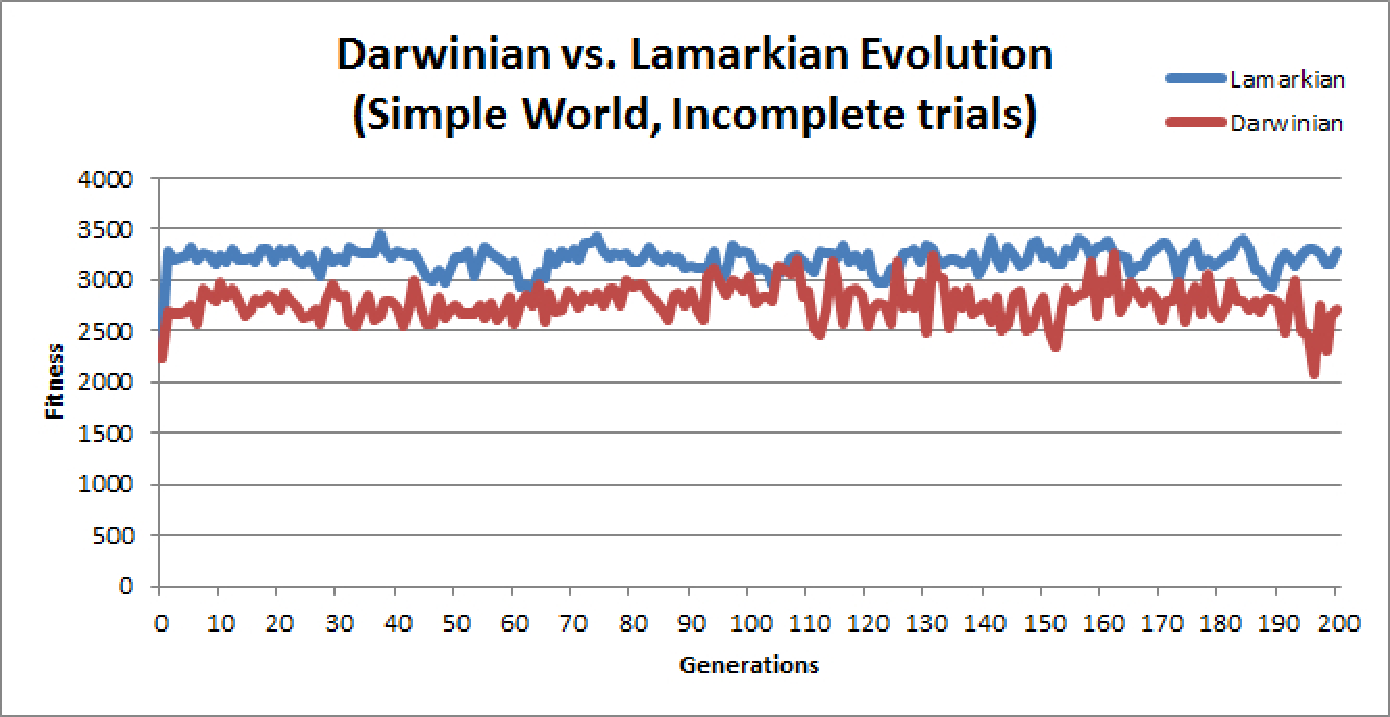
\includegraphics[scale=.35]{darwinian_vs_lamarkian_evolution.pdf}
  \caption{Lamarkian learning is more effective than Darwinian and converges more rapidly.}
  \label{fig:darwin-lamark}
\end{figure}


Figure \ref{fig:darwin-lamark} shows the results of applying our reward-based social learning algorithm to the foraging domain for both the Lamarkian and Darwinian paradigms. The performance of both algorithms quickly converges, with Lamarkian converging to a higher solution than Darwinian evolution. In the context of \textit{on-line} evolutionary learning algorithms, previous work \cite{whiteson2006evolutionary} has shown that Darwinian evolution is likely to be preferable to Lamarkian evolution in dynamic environments where adaptation is essential and the Baldwin effect \cite{simpson1953baldwin} may be advantageous. However, as adaptation is not necessary for our agents (i.e., the rewards of each plant type are the same in every generation), it seems reasonable that Lamarkian evolution outperforms Darwinian evolution.

Nevertheless, in both cases performance converges to a lower score than that of our baseline neuroevolution. We next present the results of introducing culture into reward-based social learning to overcome premature convergence.

\subsection*{Population vs. Cultural Learning}
While Lamarkian social learning is able to find good results quickly, it is likely to provide redundant information and harmfully mutated agents will train all other agents in the population on bad behavior. Thus, it is likely that a mono-culture population will converge too quickly to a sub-optimal fitness as the majority drags down t

In order to address this problem, we introduce a cultural version of reward-based social learning designed to promote and protect diversity. At the start of each generation, the population is divided into 10 cliques of 10 agents each, with each agent's clique decided at random. During the evaluation, agents only teach and learn from other agents in their own clique. In addition to increasing behavioral diversity relative to learning from the entire population, this cultural variant of reward-based learning also has the appealing practical advantage that it decreases the worst-case number of iterations of backprop in a generation by a factor of ten.

\begin{figure}
  \centering
    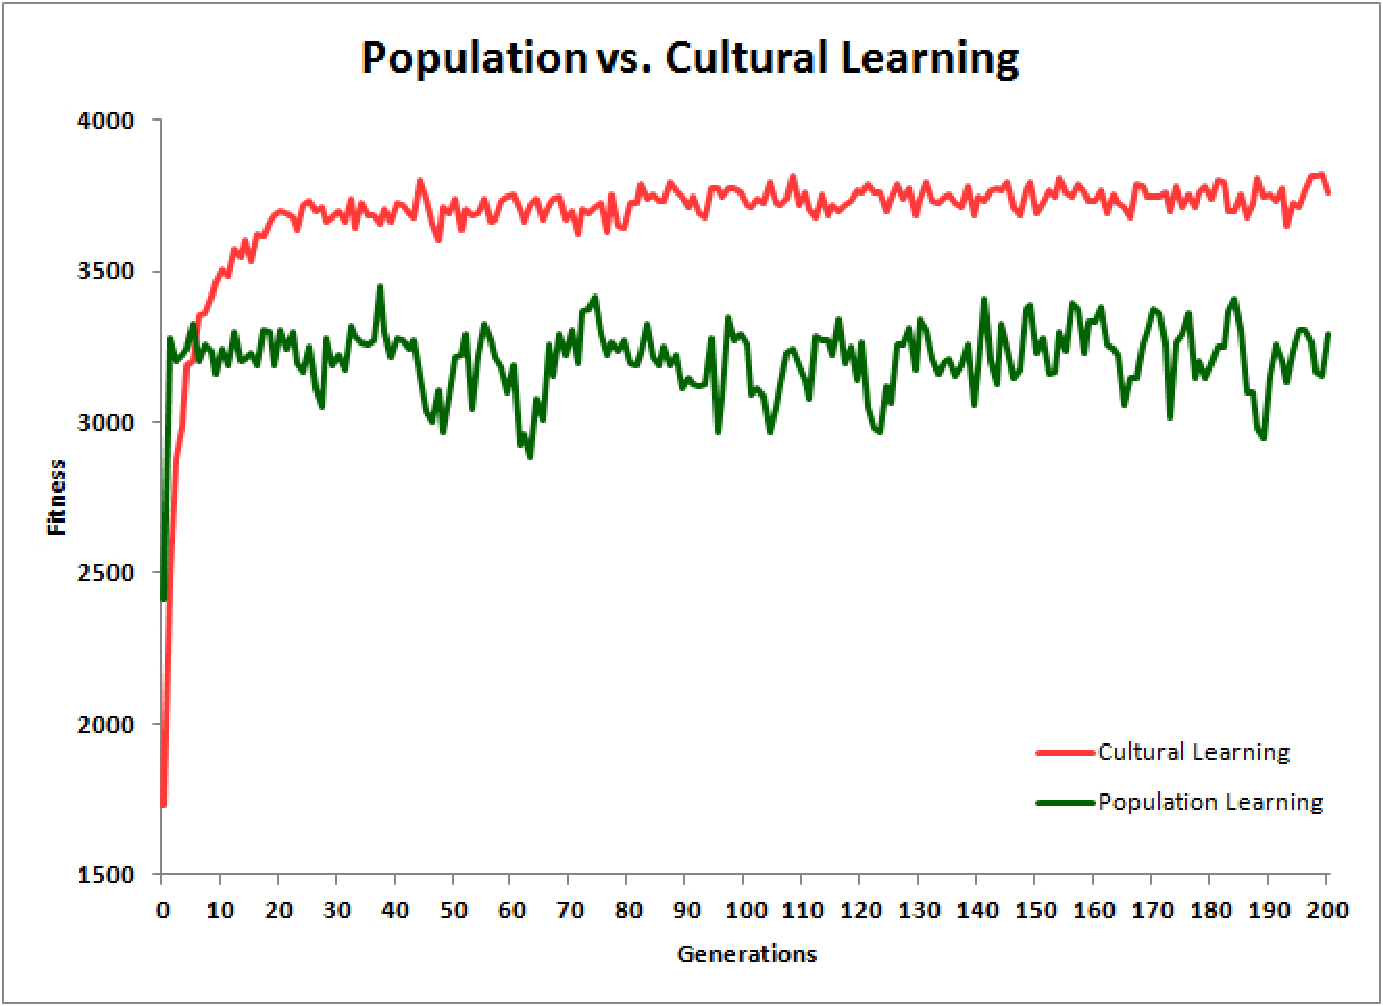
\includegraphics[scale=.35]{population_vs_cultural_learning.pdf}
  \caption{The results of agents learning from observations of the entire population compared to only agents in the same clique.}
  \label{fig:population-social}
\end{figure}

Figure \ref{fig:population-social} shows the results comparing population-based and cultural learning. The cultural social learning not only reaches a higher peak than the population based method, but also arrives at this level of fitness more rapidly than the baseline neuroevolution approach. Preventing agents who have behavior that is harmful from impacting the remainder of the population provides safety and protection; when every mutated organism has the opportunity to train every other, as is the case in population-wide learning, the entire population may be negatively impacted. Because cultural evolution is more efficient and provides better results, likely due to this protection from mutation and the fostering of diversity, we incorporate it in our final algorithm.

The next experiment compares our cultural learning algorithm to a benchmark student-teacher model.

\begin{figure}
  \centering
    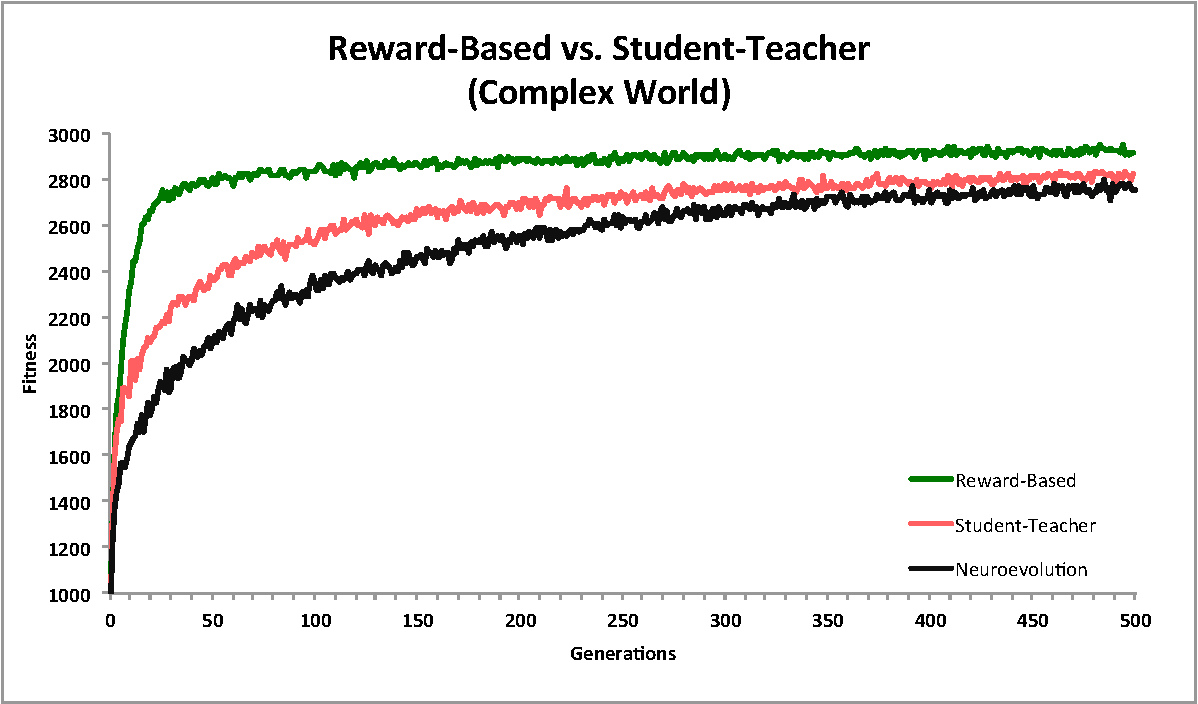
\includegraphics[scale=.35]{complex_reward_based_vs_student_teacher.pdf}
  \caption{The results of our algorithm in a complex world evaluated alongside a more traditional student-teacher model and baseline pure neuroevolution.}
  \label{fig:reward-studetteacher}
\end{figure}
\begin{figure}
  \centering
    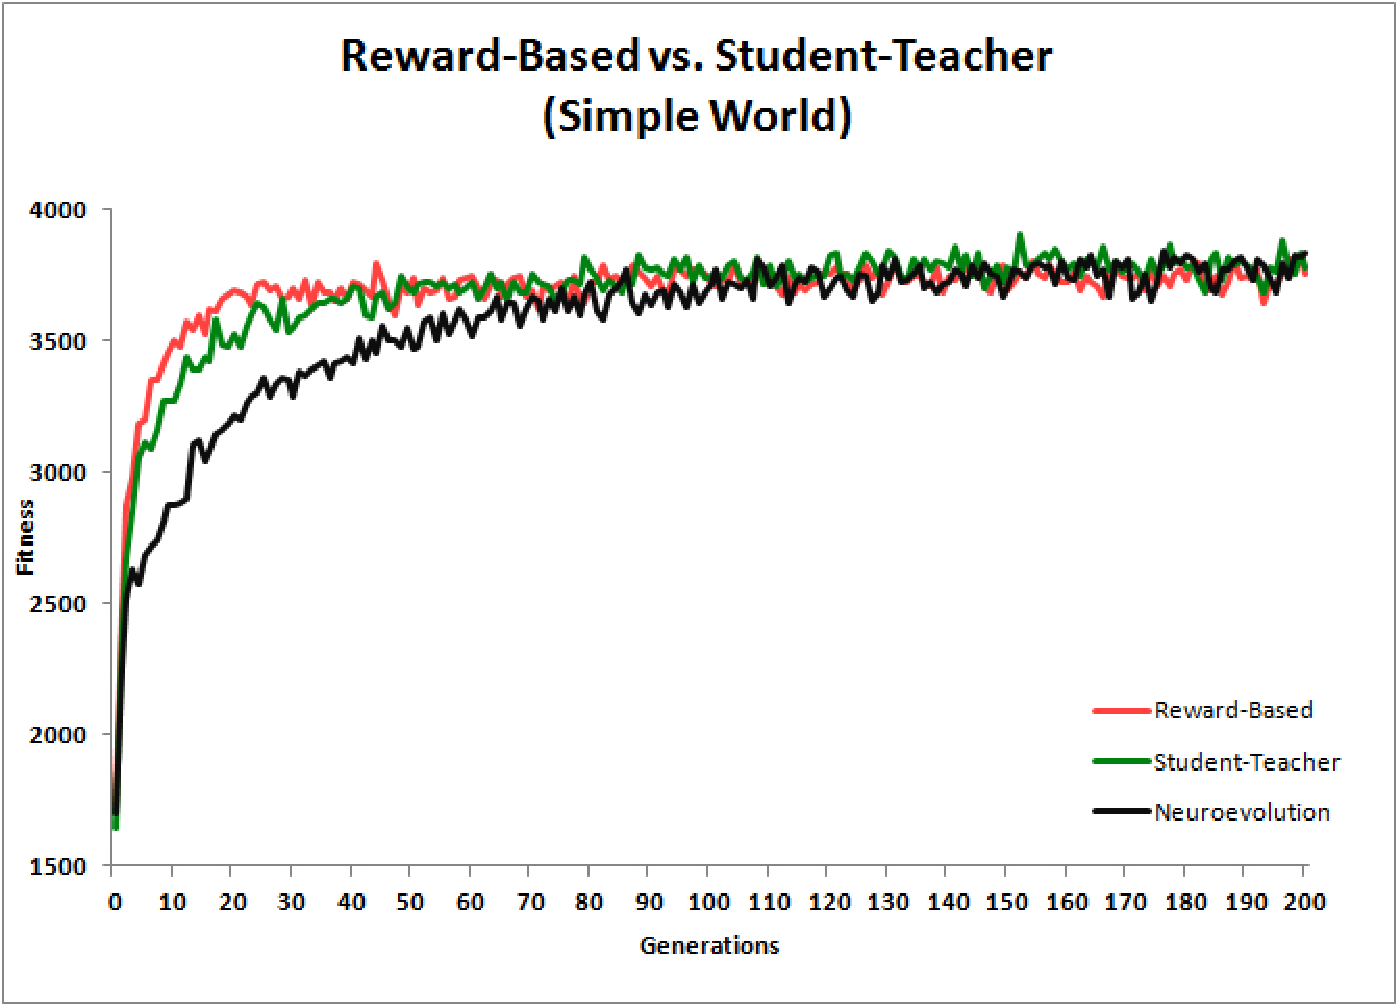
\includegraphics[scale=.35]{simple_reward_based_vs_student_teacher.pdf}
  \caption{The results of our algorithm in a simple world evaluated alongside a more traditional student-teacher model and baseline pure neuroevolution.}
  \label{fig:reward-studetteacher}
\end{figure}

\subsection*{Reward-Based Learning vs. Student-Teacher Learning}
In our final set of experiments, we compare our cultural reward-based algorithm to an on-line student-teacher learning algorithm inspired by the NEW TIES system \cite{haasdijk2008social}. The NEW TIES system utilizes a steady-state evolution in which at every timestep each agent probabilistically teaches the lowest-fitness member of that is close to it, effectively forming geographical cliques. Since the system relies on a steady-state evolution, weaker agents eventually die out and do not have as much of a chance to propagate poor training examples relative to that of long-lasting agents. To adapt this approach to our generational EA, and to maximize the fairness of our comparison, we create a population of 10 cliques with 10 agents each. At each time step, the current champion from each clique teaches its clique's lowest-fitness member.

It is worth noting that many social learning algorithms focus on off-line training, where teachers are simply the previous generation's champions. In these models, students are trained before the actual evaluation to mimic the champion(s), often with Gaussian noise added to the teacher's outputs to promote diversity in the population. However, at evaluation time these agents are static and do not learn from their own experiences or that of others. Thus, to minimize the differences in approaches, we have implemented our NEW TIES variant since it requires only a slight change in the filtering of which agents send and receive training examples.

Figure \ref{fig:reward-studetteacher} shows the results of our cultural reward-based learning algorithm compared to our student-teacher variant and pure neuroevolution. Reward-based learning converges to a near-optimal solution faster than the student-teacher variant in both the simple and the complex world. While in the simple world this speed up is slight, in the complex world our reward-based approach is more than an order of magnitude faster, reaching a higher fitness by generation 50 than either student-teacher or baseline neuroevolution achieve by generation 500.

In the next section, we present a discussion of our experimental results and indicate possible future directions for reward-based social learning.

\section{Discussion and Future Work}
\label{sec:future}
The results of our experiments in reward-based social learning clearly indicate that it has the potential to breathe new life into social algorithms.

To better understand why the cultural version of our algorithm was able to prevent premature convergence and achieve significant results, we analyzed the behavioral diversity of the population after every generation. After the evaluation phase, we generated a new instance of the simple world and created a set of input states corresponding to random locations, orientations, and velocities. For every agent, we then observed its output response (i.e., the desired change in velocity and orientation) for each of the input states. Figures \ref{fig:orientation} and \ref{fig:velocity} show the average variance of the population response to each of the 100 input states after every generation, effectively measuring the behavioral diversity of the popluation.

Although the orientation and velocity results may seem contradictory, they are actually reflecting a desirable property of cultural evolution. In the case of velocity, both the population and cultural algorithms quickly converge to low diversity. Since there is no benefit to slowing down in our current domain, one would expect a strong strategy to always output the maximum value for velocity. Thus, preserving diversity in this area would be detrimental to the performance of the population. Conversely, the diversity of orientation should be preserved, as there is a tradeoff between turning toward an immediate but small reward, such as a single plant within one step, and turning toward a delayed reward, such as a cluster of plants a few steps away. This complexity suggests that the fitness landscape for orientation  is likely filled with numerous local optima and diversity preservation should be beneficial to evolution. 

We believe the results of our diversity analysis support the hypothesis that our cultural algorithm preserves diversity only when it is useful (e.g., orientation response), while not preventing convergence when diversity is unnecessary (e.g., velocity response).

The robot foraging domain is a well-suited domain for exploring extensions and improvements to our social learning algorithm. One interesting future work direction may be to introduce obstacles or walls that block the agent from immediately receiving the reward. Where as the current problem domain only utilizes a single example at every time step, teaching more complex behaviors using reward-based approaches may require that the memory contains sequences of input-output pairs. Additionally, we have plan to introduce predators into the world and measure the effects reward-based social learning has when leveraged by either predators, prey, or both.

Finally, we plan to expand our benchmark suite to include more student-teacher variants in the future. Although we believe our experiment sufficiently demonstrated the advantages of reward-based social learning, student-teacher methods can be implemented in many ways, including off-line learning \cite{acerbi2007social}, probabilistic teaching \cite{haasdijk2008social}, and noisy examples \cite{denaro1996cultural}, to name only a few. A more complete set of benchmarks will help us better understand the relative performance of our approach.

\begin{figure}
  \centering
    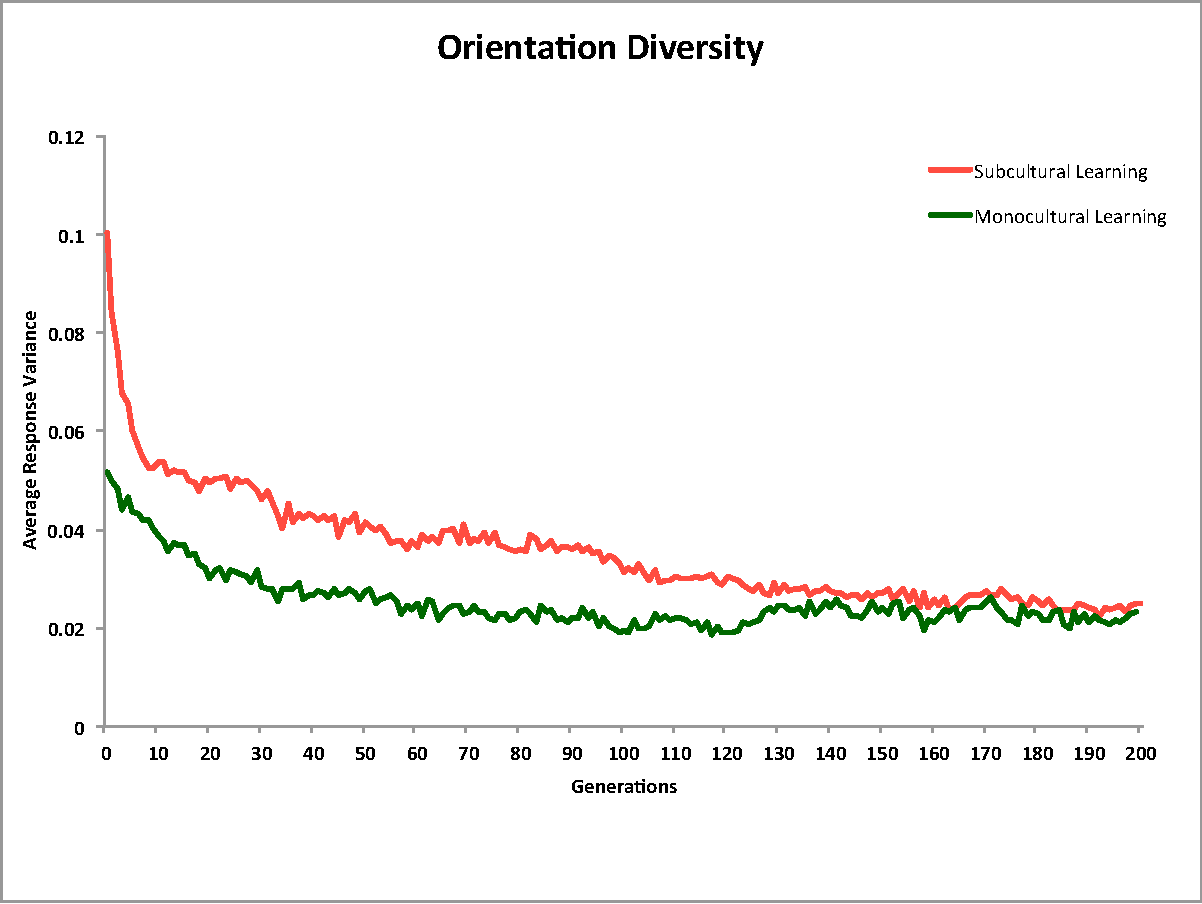
\includegraphics[scale=.35]{orientation_diversity.pdf}
  \caption{In the cultural learning model, diversity in terms of orientation is maintained for longer than in population learning before behavior converges.}
  \label{fig:orientation}
\end{figure}

\begin{figure}
  \centering
    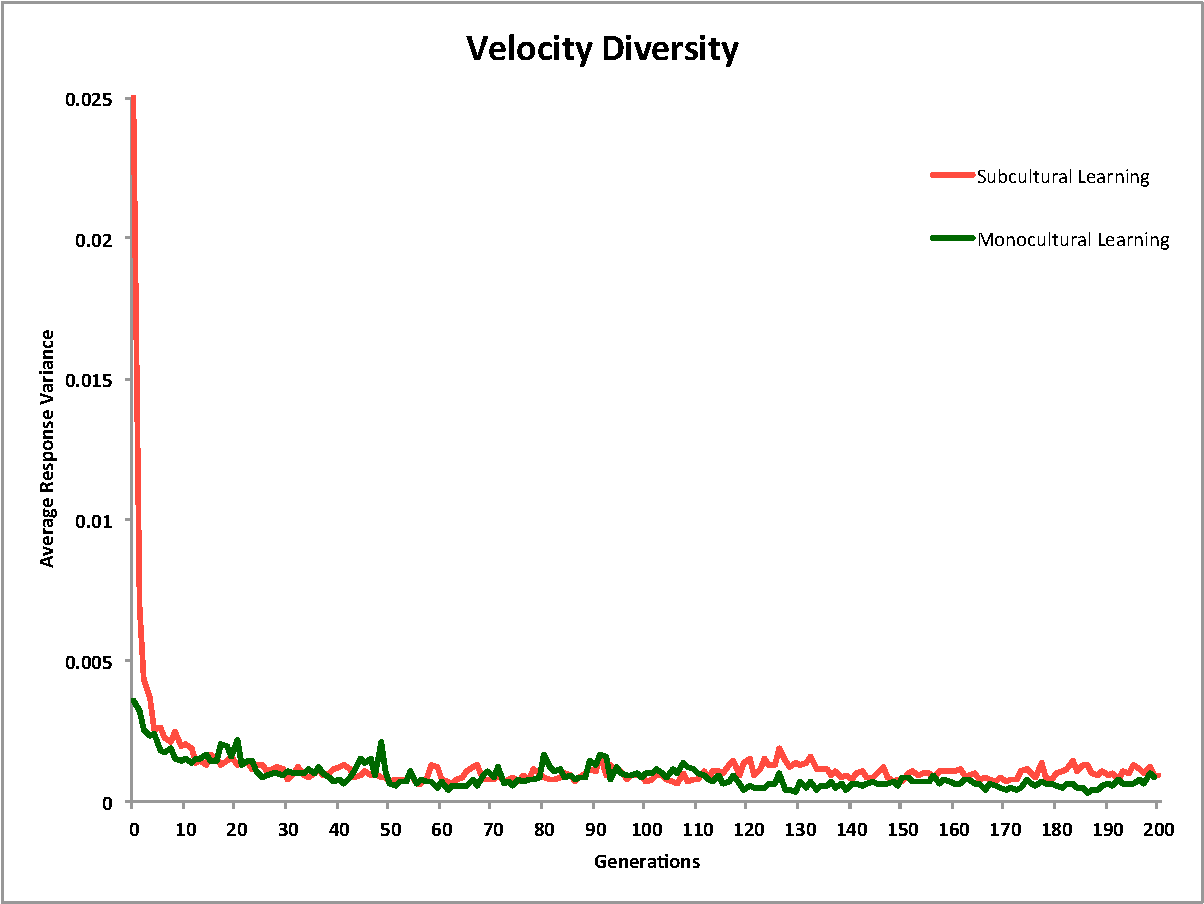
\includegraphics[scale=.35]{velocity_diversity.pdf}
  \caption{Velocity converges more quickly in the cultural model than in the population model.}
  \label{fig:velocity}
\end{figure}

Future work may involve investigating the relationship between this and other forms of social learning and Q-learning.  Additionally, one strength of non-hierarchical social learning is its ability to transmit information about novel situations to all agents without those agents having to experience those situations themselves.  As such, investigating the impact of non-hierarchical social learning in dynamic domains with changing rewards is a promising and practical avenue for new research.  Finally, our current model teaches agents about the previous timestep with one iteration of backprop whenever there is a reward.  Extending the model to account for the magnitude of the reward, and to store and train on information about previous timesteps may lead to new insights.   

\section{Conclusions}
\label{sec:conclusions}

We have presented a reward-based approach to apply social learning in evolutionary algorithms that converges to better solutions faster than previous known solutions. Traditionally, social learning in evolutionary algorithms has followed a student-teacher model that assigns roles to each agent. Our approach removes this hierarchy and instead updates individuals based on actions taken by \textit{any} agent that lead to a positive reward.  Further filtering of results by constraining teaching samples to those from the same cultural group results in further improvement to performance.  Experiments in a complex robot foraging domain demonstrate that this approach is highly effective at quickly learning a near-optimal policy with Lamarkian evolution. 

\bibliographystyle{abbrv}
\bibliography{sigproc}
\end{document}